\documentclass[11pt]{article}

% ---- Packages ---------------------------------------------------------------
\usepackage[margin=0.6in]{geometry}
\usepackage{amsmath,amssymb}
\usepackage{enumitem}
\usepackage{multicol}
\usepackage{tikz}
\usepackage{pgfplots}
\pgfplotsset{compat=1.18}
\usepackage{graphicx}
\usepackage{xcolor}
\usepackage{fancyhdr}
\usepackage{array}
\usepackage{tcolorbox}
\usepackage{wrapfig}
\usepackage{parskip}

% ---- Formatting -------------------------------------------------------------
\setlength{\columnsep}{0.35in}
\setlist[enumerate]{leftmargin=*, itemsep=8pt}
\pagestyle{fancy}
\fancyhf{}
\fancyfoot[L]{\small\textit{en}Vision\textsuperscript{\textregistered} Algebra 2}
\fancyfoot[C]{\small Topic 6 Assessment, Form B}
\fancyfoot[R]{\small\thepage}
\renewcommand{\headrulewidth}{0pt}

% ---- Helper commands --------------------------------------------------------
% Answer blank box (for fill-in answers)
\newcommand{\blankbox}[1][2.2cm]{%
  \tikz[baseline=(b.base)]\node[draw, rounded corners=2pt, minimum width=#1,
    minimum height=7mm, inner sep=2pt] (b) {\phantom{Ag}};}

% Choice bubble (filled/empty circle for MC letter)
\newcommand{\choice}[1]{%
  \tikz[baseline=-0.6ex]\node[draw, circle, inner sep=0.6pt,
    minimum size=3.3mm, font=\scriptsize\bfseries] {#1};\;}

% Select-all-that-apply square checkbox
\newcommand{\checkbox}{$\square$\;}

% Draggable-style token box (for questions 5, 8 that use option tiles)
\newcommand{\tokenbox}[1]{%
  \tikz[baseline=(t.base)]\node[draw, rounded corners=2pt,
    minimum height=7mm, minimum width=1.1cm, inner sep=3pt] (t) {$#1$};}

% Section break between questions inside columns
\newcommand{\qsep}{\par\vspace{4pt}\noindent\hrulefill\par\vspace{4pt}}

% ---- Document ---------------------------------------------------------------
\begin{document}

% =============================================================================
% STUDENT VERSION
% =============================================================================

\noindent
\textbf{Name}\; \rule{6cm}{0.4pt} \hfill \textit{\small SavvasRealize.com}

\vspace{4pt}
\noindent\rule{\textwidth}{0.6pt}

\vspace{2pt}
\noindent{\LARGE\textbf{6 \; Topic Assessment Form B}}

\vspace{6pt}
\noindent\rule{\textwidth}{0.6pt}

\vspace{8pt}

\begin{multicols}{2}

% --- Q1 (orig Q9) ---
\noindent\textbf{1.} What is the solution to the equation $\log_3(2x - 3) = -1$? Round to the nearest thousandth.

\vspace{4pt}
\noindent $x = $ \blankbox[1.8cm]

\qsep

% --- Q2 (orig Q10) ---
\noindent\textbf{2.} The graph shows the function $f(x) = 32\!\left(\tfrac{1}{2}\right)^x - 2$. What is the value of the inverse function $f^{-1}$ at $x = 2$?

\begin{center}
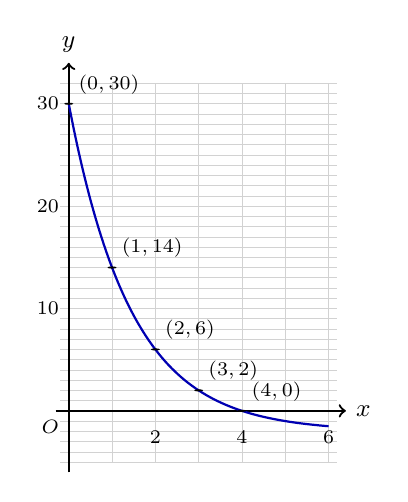
\begin{tikzpicture}[xscale=0.55, yscale=0.13]
  % Grid
  \draw[help lines, gray!35, step=1] (-0.2,-5) grid (6.2,32);
  % Axes
  \draw[->, thick] (-0.3,0) -- (6.4,0) node[right] {\small $x$};
  \draw[->, thick] (0,-6) -- (0,34) node[above] {\small $y$};
  % Tick labels
  \foreach \x in {2,4,6} \node[below, font=\scriptsize] at (\x,-1) {\x};
  \node[left, font=\scriptsize] at (0,10) {10};
  \node[left, font=\scriptsize] at (0,20) {20};
  \node[left, font=\scriptsize] at (0,30) {30};
  \node[below left, font=\scriptsize] at (0,0) {$O$};
  % Curve: f(x) = 32*(1/2)^x - 2
  \draw[thick, blue!70!black, domain=0:6, samples=60, smooth]
    plot (\x, {32*pow(0.5,\x) - 2});
  % Labeled points
  \fill[black] (0,30) circle (3pt) node[above right, font=\scriptsize] {$(0, 30)$};
  \fill[black] (1,14) circle (3pt) node[above right, font=\scriptsize] {$(1, 14)$};
  \fill[black] (2,6) circle (3pt) node[above right, font=\scriptsize] {$(2, 6)$};
  \fill[black] (3,2) circle (3pt) node[above right, font=\scriptsize] {$(3, 2)$};
  \fill[black] (4,0) circle (3pt) node[above right, font=\scriptsize] {$(4, 0)$};
\end{tikzpicture}
\end{center}

\vspace{2pt}
\noindent $f^{-1}(2) = $ \blankbox[1.8cm]

\qsep

% --- Q3 (orig Q7) ---
\noindent\textbf{3.} What function is the inverse of the exponential function $y = \left(\tfrac{1}{3}\right)^x$?

\begin{itemize}[label=\null, leftmargin=1.2em, itemsep=2pt, topsep=2pt]
  \item \choice{A} $y = x^{\tfrac{1}{3}}$
  \item \choice{B} $y = \left(\tfrac{1}{3}\right)^x$
  \item \choice{C} $y = \log_{\tfrac{1}{3}} x$
  \item \choice{D} $y = \log_x \left(\tfrac{1}{3}\right)$
\end{itemize}

\qsep

% --- Q4 (orig Q11) ---
\noindent\textbf{4.} What is the asymptote of the graph of $g(x) = \log_2(x + 4)$?

\begin{itemize}[label=\null, leftmargin=1.2em, itemsep=2pt, topsep=2pt]
  \item \choice{A} vertical at $x = 0$
  \item \choice{B} vertical at $x = -4$
  \item \choice{C} horizontal at $y = 0$
  \item \choice{D} horizontal at $y = -4$
\end{itemize}

\qsep

% --- Q5 (orig Q12) ---
\noindent\textbf{5.} Complete the equation of the inverse of the function $f(x) = \log_4(3x)$.

\begin{center}
\tokenbox{4} \quad \tokenbox{\tfrac{1}{3}} \quad \tokenbox{\tfrac{1}{4}} \quad \tokenbox{3}
\end{center}

\vspace{2pt}
\noindent $f^{-1}(x) = $ \blankbox[1.2cm] $\Big($ \blankbox[1.2cm] $\Big)^{x}$

\qsep

% --- Q6 (orig Q13) ---
\noindent\textbf{6.} Use the properties of logarithms to choose the expression $x\log 2 - \log\tfrac{1}{3}$ as a single logarithm.

\begin{itemize}[label=\null, leftmargin=1.2em, itemsep=2pt, topsep=2pt]
  \item \choice{A} $\log\!\left(2x - \tfrac{1}{3}\right)$
  \item \choice{B} $\log\!\left(\tfrac{2}{3x}\right)$
  \item \choice{C} $\log\!\left(2^x - \tfrac{1}{3}\right)$
  \item \choice{D} $\log(3(2)^x)$
\end{itemize}

\qsep

% --- Q7 (orig Q14) ---
\noindent\textbf{7.} The profit for a new website, in thousands of dollars, can be represented by $5^x$, where $x$ is time in months. Find the time when the company's profit is \$15{,}000. Select the exact solution as a logarithm, and select an approximate solution.

\begin{itemize}[label=\null, leftmargin=1.2em, itemsep=2pt, topsep=2pt]
  \item \checkbox \textbf{A.} $x = \log_{15} 5$
  \item \checkbox \textbf{B.} $x = \log_{5} 15$
  \item \checkbox \textbf{C.} $x = \log 15$
  \item \checkbox \textbf{D.} $x = 1.689$
  \item \checkbox \textbf{E.} $x = 0.594$
  \item \checkbox \textbf{F.} $x = 0.176$
\end{itemize}

\qsep

% --- Q8 (orig Q16) ---
\begin{minipage}{\linewidth}
\noindent\textbf{8.} Complete the steps to write the expression $2\log a + 2\log b - 3\log c$ as a single logarithm using the properties of logarithms.

\begin{center}
\tokenbox{\text{Product}} \quad \tokenbox{\text{Quotient}} \quad \tokenbox{\text{Power}}
\end{center}

\begin{align*}
&\; 2\log a + 2\log b - 3\log c \\
&= \log a^{2} + \log b^{2} - \log c^{3} \quad \blankbox[1.7cm]\\
&= \log a^{2}b^{2} - \log c^{3} \quad \blankbox[1.7cm]\\
&= \log\!\left(\frac{a^{2}b^{2}}{c^{3}}\right) \quad \blankbox[1.7cm]
\end{align*}
\end{minipage}

\end{multicols}

\clearpage

% =============================================================================
% TEACHER ADDENDUM — ANSWER KEY
% =============================================================================

\begin{center}
  {\Large\bfseries Addendum — Teacher Answer Key}\\[3pt]
  {\small Topic 6 Assessment, Form B \;\textbullet\; \textit{en}Vision\textsuperscript{\textregistered} Algebra 2}
\end{center}

\vspace{6pt}
\hrule
\vspace{10pt}

\begin{enumerate}[leftmargin=2.1em, itemsep=7pt]

\item $x = \boxed{1.667}$ \\
\textit{$\log_3(2x - 3) = -1 \Rightarrow 2x - 3 = 3^{-1} = \tfrac{1}{3} \Rightarrow 2x = \tfrac{10}{3} \Rightarrow x = \tfrac{5}{3} \approx 1.667$.}

\item $f^{-1}(2) = \boxed{3}$ \\
\textit{From the graph, $f(3) = 2$; therefore $f^{-1}(2) = 3$.}

\item \textbf{C} \quad $y = \log_{\frac{1}{3}} x$ \\
\textit{The inverse of $y = b^x$ is $y = \log_b x$.}

\item \textbf{B} \quad vertical at $x = -4$ \\
\textit{A log function $\log_2(x + 4)$ is undefined when $x + 4 = 0$, giving a vertical asymptote at $x = -4$.}

\item $f^{-1}(x) = \boxed{\tfrac{1}{3}} \, (\,\boxed{4}\,)^{x}$ \\
\textit{If $y = \log_4(3x)$, then $4^y = 3x$, so $x = \tfrac{1}{3}(4)^y$. Swapping variables: $f^{-1}(x) = \tfrac{1}{3}(4)^x$.}

\item \textbf{D} \quad $\log(3(2)^x)$ \\
\textit{$x\log 2 - \log\tfrac{1}{3} = \log 2^x - \log \tfrac{1}{3} = \log\!\left(\dfrac{2^x}{1/3}\right) = \log(3 \cdot 2^x)$.}

\item \textbf{B} \; $x = \log_5 15$ \; and \; \textbf{D} \; $x \approx 1.689$ \\
\textit{$5^x = 15 \Rightarrow x = \log_5 15$, which is approximately $1.689$ as rounded in the answer key.}

\item Steps (in order): \textbf{Power}, \textbf{Product}, \textbf{Quotient}.
\begin{align*}
2\log a + 2\log b - 3\log c &= \log a^{2} + \log b^{2} - \log c^{3} &&\text{(Power)}\\
&= \log(a^{2}b^{2}) - \log c^{3} &&\text{(Product)}\\
&= \log\!\left(\frac{a^{2}b^{2}}{c^{3}}\right) &&\text{(Quotient)}
\end{align*}

\end{enumerate}

\vspace{12pt}
\hrule
\vspace{4pt}
\noindent{\footnotesize
Answer key reflects Savvas \textit{en}Vision Algebra 2, Topic 6 Assessment Form B, Assessment Sourcebook.
Explanations are supplemental notes for instructor reference.}

\end{document}
